%!TEX root = thesis.tex

\chapter{User Study}
\label{chap:user-study}

A second lab study was conducted to test the impact of additional visual feedback (beyond the raw source code) on audience understanding and enjoyment in live coding.

It was hypothesised that the didactic visualisation (see Section~\ref{sec:didactic-visualisation}) approach would result in
enhanced audience understanding, and a reduction in audience confusion
through the performance. In contrast, it was predicted that the aesthetic
visualisations (see Section~\ref{sec:aesthetic-visualisation}) would positively influence audience enjoyment, both overall and over the course of the performance.

%%%%%%%%%%%%%%%% Inital Report for study

% Two code visualisations have been analysed in a live coding context to determine effective presentational and educational features. Two visualisations were evaluated including a visualisation targeting aesthetic appeal and a visualisation with a more didactic approach. The goal was to determine the usability, differences and desirability of the two approaches to further inform future live coding visualisations.\\

% The set of didactic visualisations predominantly focussed on the relationship between the live coding active processes and their behaviour. The visualisations prominently displaying the names of the active functions with visual indication of the number of functions running and their callback time. Bright colours and solid shapes were used to ensure constant visibility and communicate the intention of the underlying code. Overall, four visualisations were presented with each introduced depending on the number of active functions. It was predicted that taking a more educational approach would see a reduction in audience confusion through the performance.\\

% The set of aesthetic visualisations focussed less on the programmatic aspects of the live coding performance, rather intending to provide additional visual interest to the projected code thereby prolonging attention. More variety was used in visual structure and colour. Again, four visualisations were presented, varying the visualisation based on the number of active functions. It was predicted that focussing on the aesthetic nature of the visualisations would assist in audience retention and result in a consistency of interest through the performance.


\section{Method}

Two independent audiences ($N=19+22=41$) recruited through an on-campus advertisement each watched a live coder perform two ten-minute ``sets'': one accompanied by the didactic visuals, and one with the aesthetic. The order of presentation of the two visual conditions was swapped between the groups. The improvisational nature of a live coding performance makes ``controlled'' experiments difficult, but the live coding artist attempted (as much as possible) to do the same two performances for each group.

Over the course of these performances, each audience member completed a survey consisting of four sections: demographic information, their opinion of the first piece, their opinion of the second piece and questions about the performance overall. Similar to the first field trial, the questionnaire primarily focussed on self-reported levels of ``enjoyment'' and ``understanding'' related to the visualisations specifically and also to the performance more generally. There was also a free-form question for suggested improvements to the visualisations.

After the lab study performance, a
video-cued-recall~\cite{Suchman1992} interview was conducted with
the live coder using a video of the performance.

% Two sets of visualisations were presented to an audience during a live coding performance and surveys were distributed. The performance was run as two ten minute improvised songs with each song demonstrating one of the two experimental visualisation conditions, either the didactic condition or the aesthetic condition. The experiment was run twice, with two separate participant groups, swapping the order in which the two sets of visualisations were presented to the audience.\\

% The audience members completed a survey (see Appendix B) consisting of four sections over the course of the performance. These sections included a demographic information section, opinion of the first visualisation, opinion of the second visualisation and a section investigating the audience's overall opinion of the performance. The sections regarding the visualisations predominantly focussed on the enjoyment and understanding related to the visualisation while the final section focussed on eliciting potential improvements.\\

% After explaining to the participants the structure of the experiment and allowing the participants to complete the initial demographic section of a survey, the live coder began the first performance utilising one of the two visualisations. Following this first set, the second section of the survey was conducted. A second set was then played using the alternative visualisation. Following this second set, the same survey questions were administered again, again asking the participants specifics about their enjoyment and understanding related to the specific visualisation demonstrated. A final survey question was then asked relating to their opinion regarding the whole performance and their suggested improvements.\\

% To further inform the outcomes of the experiment a video-cued recall interview was conducted following the performance with the live coder. Two of the performances were examined critically and further discussion concerning the advantages and limitations of the visualisations were examined.

\section{Participants}

Of the 41 participants that took part in the study over the two performances, 19 participants observed the first performance and 22 participants observed the second performance. The demographic makeup of the audiences was similar.

$66\%$ of the participants were male (see Figure \ref{genderdistribution}) and most participants were aged between 18 and 32 ($76\%$, see Figure \ref{agedistribution}). As the study was conducted within the Computer Science Department, a large proportion of the participants were experienced with programming with $90\%$ having current or previous experience with it (see Figure \ref{programmingdistribution}). Nevertheless, only $15\%$ of participants had previous experience with any of the Lisp style of languages (see Figure \ref{lispdistribution}), the style used within the performance.

Of the participants, $68\%$ stated that they listened to a large amount of music (see Figure \ref{musicdistribution}) though only about $15\%$ of participants stated that they played an instrument or sung regularly (see Figure \ref{instrumentdistribution}). $78\%$ of the participants had never seen a live coding performance before.

\section{Results}

The audience-reported enjoyment and understanding responses from the questionnaire were evaluated for the two visualisation conditions as described below. A significance level of $0.05$ was used for the Chi-squared analysis.

\subsection{Enjoyment}

\afterpage{
\begin{figure}
  \centering
  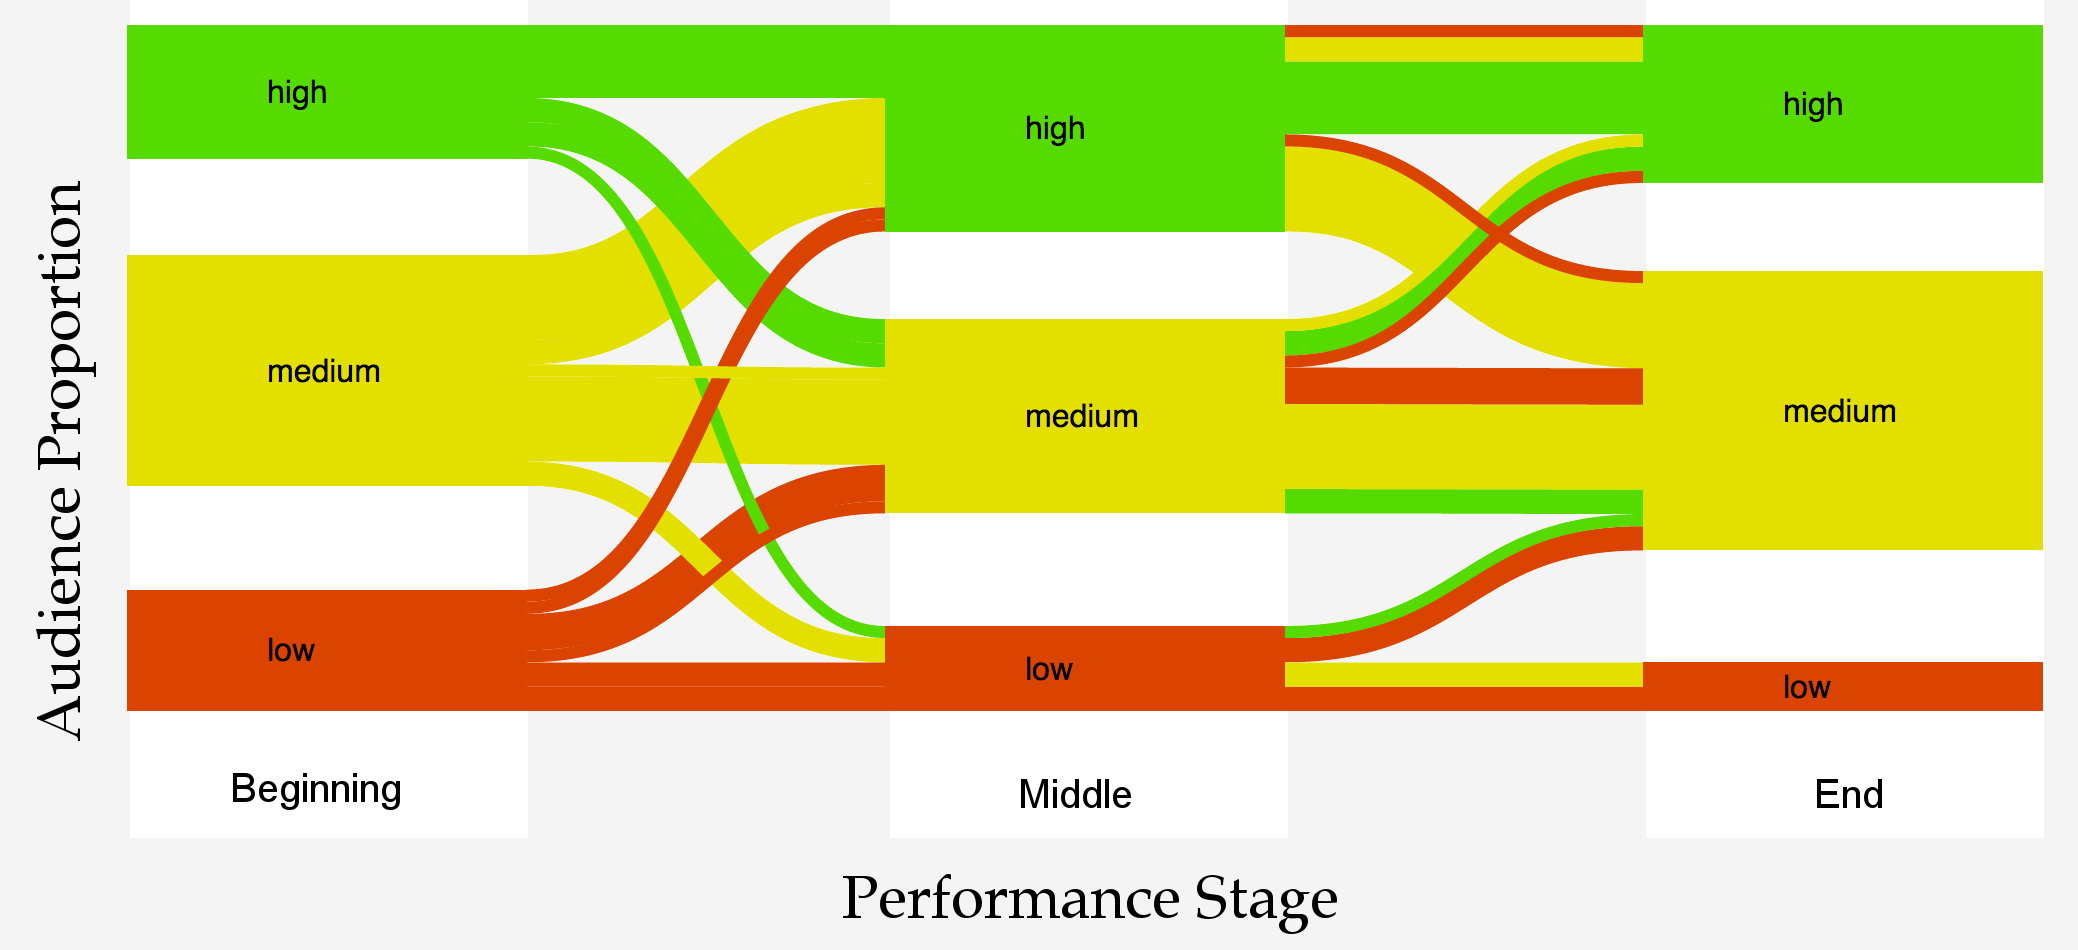
\includegraphics[width=\columnwidth]{../study-2/results/graphs/didactic-enjoyment-final}
  \caption{Audience reported enjoyment during the beginning, middle and end of the performance for the \textbf{didactic} condition. Line width at each stage indicates proportion of the audience reporting high, medium or low enjoyment, and line colour is determined by the enjoyment level at the \emph{beginning} of the performance.}
  \label{fig:didactic-enjoyment}
\end{figure}

\begin{figure}
  \centering
  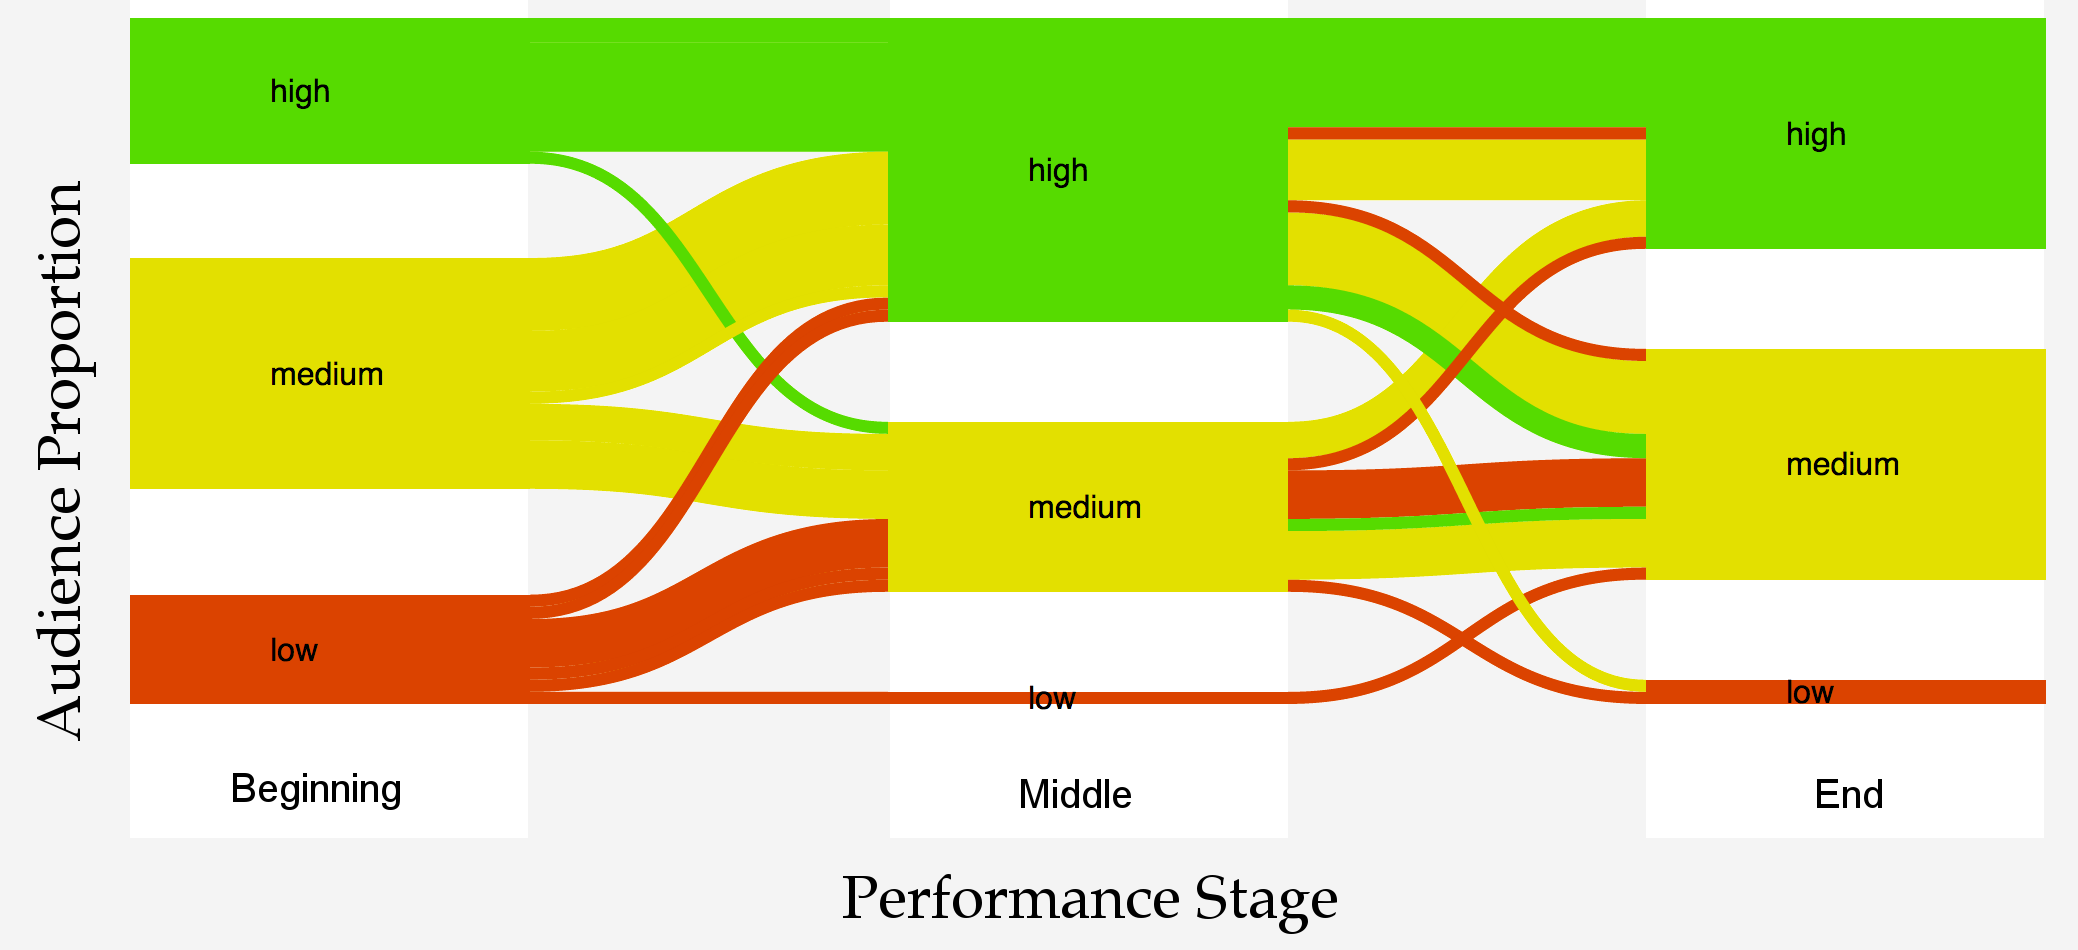
\includegraphics[width=\columnwidth]{../study-2/results/graphs/aesthetic-enjoyment-final}
  \caption{Audience-reported enjoyment level during the beginning,
    middle and end of the performance for the \textbf{aesthetic} condition.}
  \label{fig:aesthetic-enjoyment}
\end{figure}
\clearpage}

Overall, the majority of the participants reported that both visualisation conditions had a positive effect on their \textbf{enjoyment} of the performance: $76\%$ stated that the aesthetic visualisations improved their enjoyment and $56\%$ stated that the didactic visualisations improved their enjoyment. No significant difference between the visualisation types regarding  enjoyment was found ($\chi^2=3.7733,df=2,p=0.1516$).

Participants were asked to rate their enjoyment during the (self-determined) ``beginning'', ``middle'' and ``end'' of the performances (see Figure~\ref{fig:aesthetic-enjoyment} and Figure~\ref{fig:didactic-enjoyment}). During the didactic performance, $15\%$ of the audience stated that their enjoyment \emph{increased} from the beginning of the performance and was steady thereafter. By contrast, $24\%$ of the audience reported this pattern of enjoyment during the aesthetic performance. Approximately $30\%$ of the audience of all (aesthetic and didactic) performances stated that their enjoyment remained steady throughout.

\subsection{Understanding}

\afterpage{
\begin{figure}
  \centering
  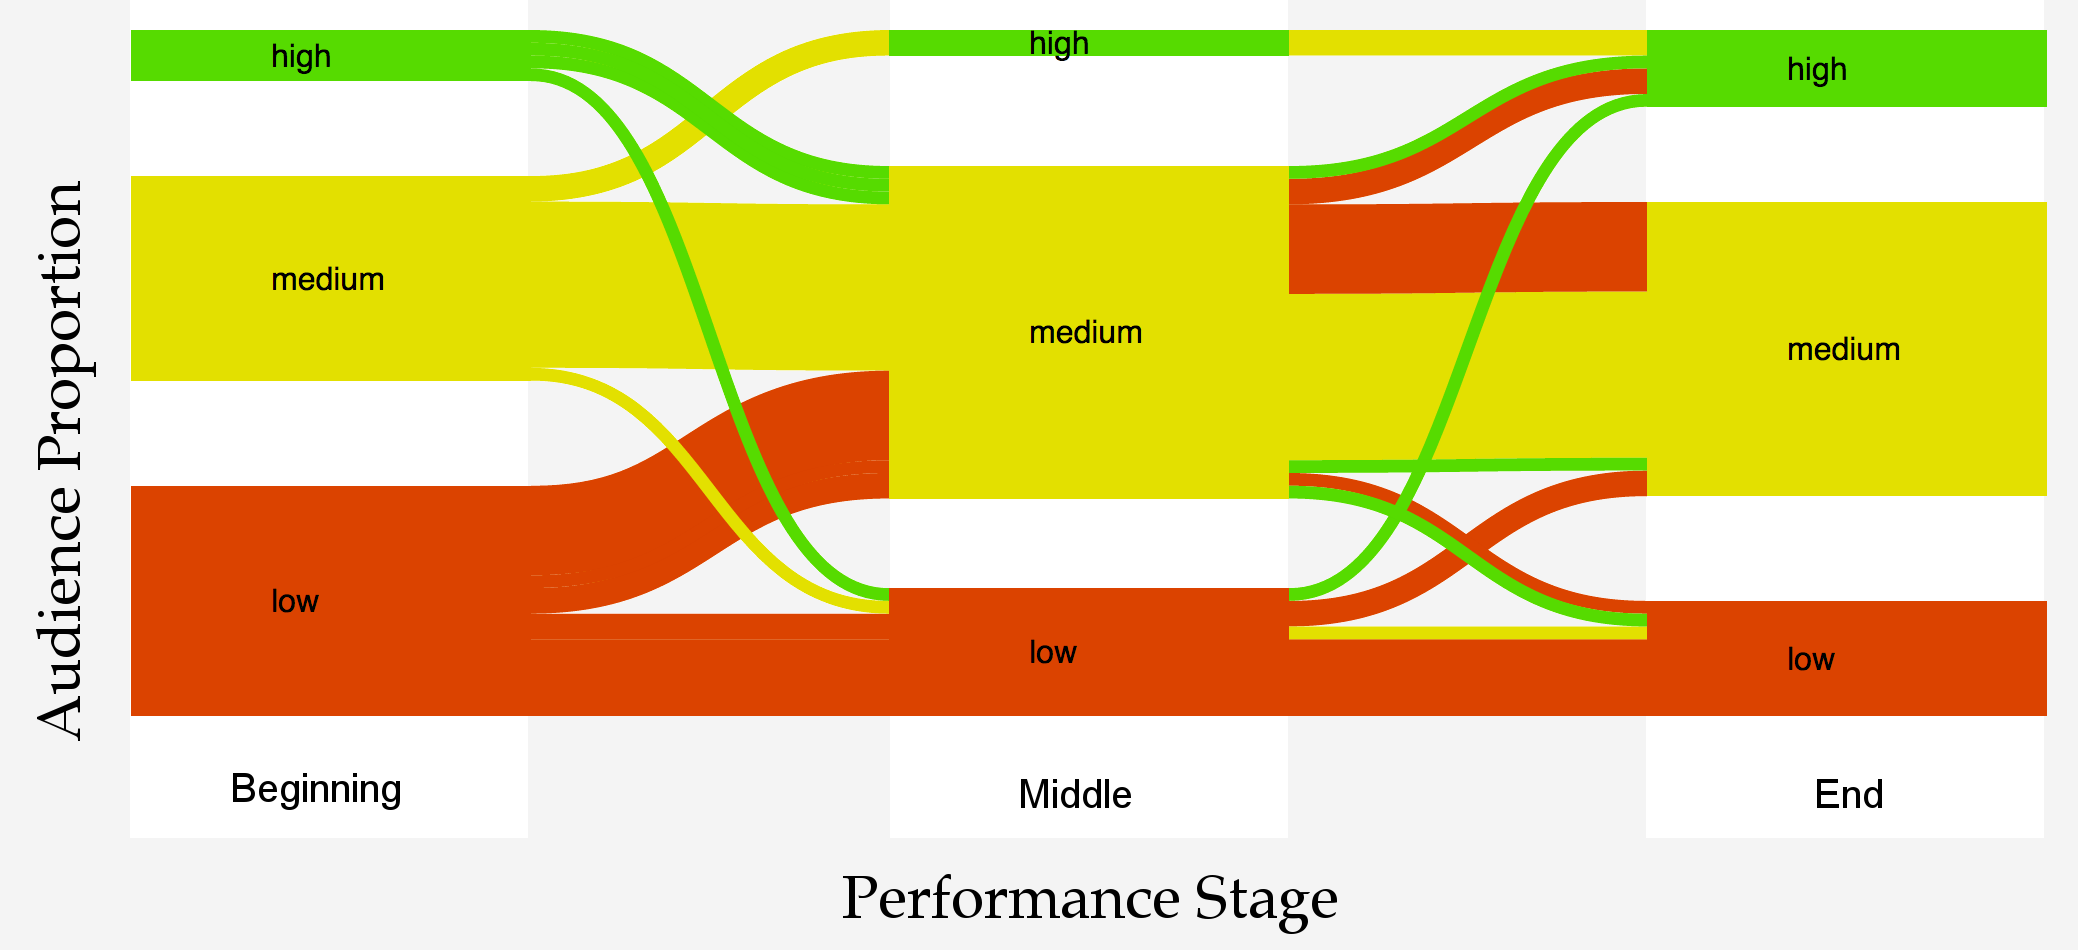
\includegraphics[width=\columnwidth]{../study-2/results/graphs/didactic-understanding-final}
  \caption{Audience reported understanding during the beginning, middle
    and end of the performance for the \textbf{didactic} condition.}
  \label{fig:didactic-understanding}
\end{figure}

\begin{figure}
  \centering
  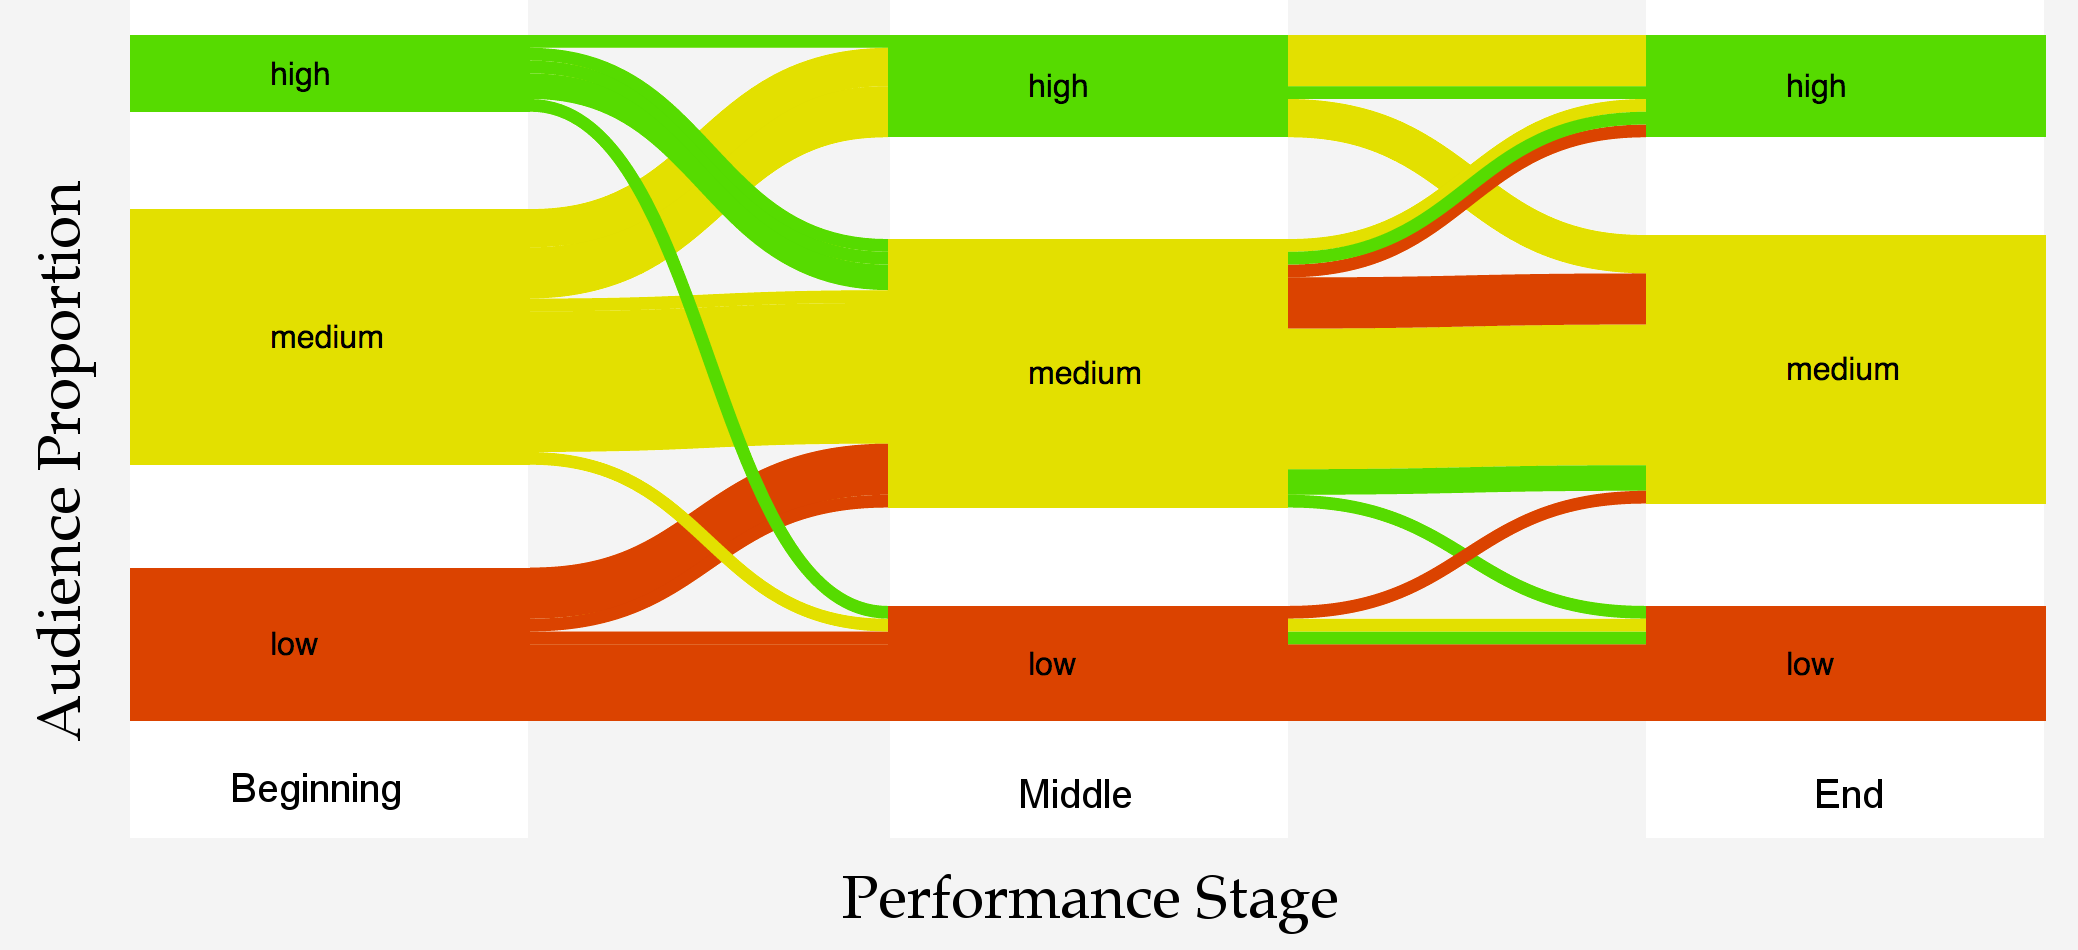
\includegraphics[width=\columnwidth]{../study-2/results/graphs/aesthetic-understanding-final}
  \caption{Audience reported understanding during the beginning, middle
    and end of the performance for the \textbf{aesthetic} condition.}
  \label{fig:aesthetic-understanding}
\end{figure}

\clearpage
}

In response to a specific survey question, $37\%$ of participants stated that overall, the didactic visualisations ``helped them to \textbf{understand} the code'', compared to $12\%$ of participants for the aesthetic visualisations. This was a significant difference between the visualisation conditions ($\chi^2=7.1986,df=2,p=0.02734$).

Again, participants were asked to rate their understanding during the (self-reported) ``beginning'', ``middle'' and ``end'' of the performance (see Figure~\ref{fig:aesthetic-understanding} and Figure~\ref{fig:didactic-understanding}). During the didactic and aesthetic performances, $49\%$ and $44\%$ respectively of the participants stated that their understanding \emph{remained the same} throughout the performances. During the didactic performance, $10\%$ of the audience reported a level of understanding that \emph{trended   downwards} (eg. high to low) compared to $20\%$ of the audience during the aesthetic performance. However, this reported advantage of the didactic visualisations was offset by the reported audience understanding at the beginning of the performance where $44\%$ indicated a low understanding with the didactic visualisations compared to only $30\%$ with the aesthetic visualisations. 

Overall, the questionnaire results for audience understanding are complex, and reported levels of understanding fluctuated during the performances. Dramatically, Figure~\ref{fig:didactic-understanding} shows that a very small proportion of the audience reported high understanding during the middle of the performances. One interpretation of this result might be that it took audience members some time to work out what the didactic visualisations were actually showing, and that this conflicted with the first impressions of what some audience members (hence the decrease in levels of understanding from beginning to middle). However, once they finally understood the graphics some audience members were then able to better understand the live-coding performance.


\subsection{Liveness}

Participants were asked to discuss how each visualisation influenced or impacted the liveness of the performance. Concepts identified included positive and negative valence towards the didactic visualisations, positive and negative valence towards the aesthetic visualisations and the relevance of visual source code. 

within the discussion included the positive and negative aspects of the didactic visualisations, the positive and negative aspects of the aesthetic visualisations, source code discussion and statements indicating an understanding between the visuals and the source code.

Overall, $54\%$ of the audience indicated negative valence towards the didactic visualisation regarding liveness referencing a variety of reasons including that the ``visuals only responded to what was typed'', that the ``musical forms didn't occur at the most expected times'' and that the visualisations ``perhaps made the performance seem too polished''.

On the other hand, $34\%$ of the audience indicated positive valence towards the didactic visualisations suggesting that ``it was easier to follow this visualisation than the code'', ``the visualisations clearly showed the changes being made to the code'' and that these visualisations ``helped more with communicating that the performance was live''.

$40\%$ of the audience had negative valence towards the aesthetic visualisation its effect on the sense of liveness. Reasons cited include that the ``influence is not clear'' between the code and the visuals, that ``the visualisation did not make much sense'' and that the ``visualisations did nothing to suggest that the performance was live''.

$32\%$ had positive valence towards the aesthetic visualisation. A variety of the response included that these visuals were ``less dominating and more complementary'' and that ``the visualisations helped to show when a piece of code started working''.

A relatively large proportion ($28\%$) of the audience discussed the importance of the source code to the sense of liveness of the performance such as that the ``code showed what the musician was doing physically''. A further $5\%$ of the audience demonstrated a deeper understanding of the live coding process such as ``changing values produced changes in tone and speed of the music pitch''.

\subsection{Improvements}

The audience was asked to indicate possible improvements to the visualisations. 40\% of the audience suggested improvements that indicate a desire to see a better relationship between the visualisations and the music, with suggestions such as matching the visualisations to musical rhythms or pitch. For example, one audience member stated that the visualisations should ``perhaps have a stronger correlation with hush tones and defined shapes, baselines with wide and soft shapes with animations that follow the beat more consistently''.

Other members of the audience stated that they would like to see a better relationship between the code and the visuals. For example, one audience member stated that ``it would be really cool once you edit a code line and then activate it for it to morph into a visualisation for as long as this line of code is active''. Another audience member stated that ``it would be better to not just relate the function to the sound but relate every beat to the sound or to the code responsible for that beat''.

Other suggestions included increasing the readability of source code, increased immediacy of actions, increasing uniformity between the visualisations and the use of images to assist with the understanding of high level concepts.



% Understanding and enjoyment were evaluated against the didactic and aesthetic visualisations. Results and statistical analysis of the differences between the aesthetic and didactic conditions follows. Note that for the following statistical analysis a significance level of $0.05$ was used with the chi-squared test for independence.

% \subsection{Understanding}

% Overall, $37\%$ participants stated specifically that the didactic visualisations helped them to understand the code, whereas $12\%$ participants stated that the aesthetic visualisations assisted in understanding the code.\\

% $H_0$: There is no difference between the aesthetic visualisations and didactic visualisations in terms of understanding.\\
% $H_1$: There is a difference between the two visualisations in terms of understanding.\\

% A significant difference between the visualisations effect on understanding was found ($\chi^2=7.1986,df=2,p=0.02734$).

% \subsection{Enjoyment}
% Overall, for both visualisations, a large proportion ($> 50\%$) of the participants stated that the visualisations helped their enjoyment of the performance. Of the participants, $76\%$ stated that the aesthetic visualisations helped their enjoyment compared to $56\%$ participants that stated the didactic visualisations helped their enjoyment.\\

% $H_0$: There is no difference between the aesthetic visualisations and didactic visualisations in terms of enjoyment.\\
% $H_1$: There is a difference between the two visualisations in terms of enjoyment.\\

% No significant difference between the two visualisations effect on enjoyment was found ($\chi^2=3.7733,df=2,p=0.1516$).

% \subsection{Change in Understanding}

% Participants were asked to rate their understanding during the beginning, middle and end of the performance.\\

% During the didactic and aesthetic performances, $49\%$ and $44\%$ of the participants respectively stated that their understanding remained the same throughout the performance.\\

% During the didactic performance, $10\%$ of the audience had an understanding that tended downwards (eg. high to low) compared to $20\%$ of the audience during the aesthetic performance meaning fewer audience members had a reduction in understanding through the didactic performance.\\

% \subsection{Change in Enjoyment}

% Participants were asked to rate their enjoyment during the beginning middle and end of the performance.\\

% During the didactic performance, $15\%$ of the audience stated that enjoyment increased during the beginning remaining steady for the remainder whereas $24\%$ of the audience said the same during the aesthetic performance.\\

% During the didactic performance, $22\%$ of the audience stated that their enjoyment decreased during the start of the performance whereas only $2\%$ stated the same for the aesthetic performance.\\

% Approximately $30\%$ of the audience during both the aesthetic and didactic performances stated that their enjoyment remained steady throughout.\\

% See Figure \ref{aestheticenjoymentchange} and Figure \ref{didacticenjoymentchange} for the distribution of changes to enjoyment between the aesthetic and didactic visualisations.\\

% \subsection{Follow-Up Interview}

% A follow-up interview was conducted with the live coder to further examine the visualisation approach taken and the overall usability of the visualisations. See Appendix D for the full interview transcript.

\section{Discussion}

The overall enjoyment of the visualisations was high, for both the aesthetic and didactic visualisations. Reported enjoyment of the aesthetic visualisations was higher than for the didactic visualisations but the trends across Figures~\ref{fig:aesthetic-enjoyment} and~\ref{fig:didactic-enjoyment} are complex.
 
As discussed above, the small number of high responses for understanding during the middle of the didactic performances, and the decreasing trend from high to middle level understanding from beginning to middle of the performances perhaps indicates a higher cognitive load for understanding the didactic visualisations themselves. In fact, features of the didactic visualisation were reported to confuse some members of the audience, despite their stated aim of \emph{assisting} audience understanding. One audience member even stated that they ``found them distracting'' and that they ``preferred just to read the code''.
 
The video-cued-recall interview indicated that the experience of the visualisations of the live coder and the audience was fundamentally different. While many members of the audience reported that they drifted between focussing on the music, focussing on the visualisations and focussing on the code, the live coder reported that their focus was purely on the code and the music, rarely drifting. In one particular section of the interview, the live coder stated: ``I definitely wasn't paying attention to them [the visualisations] on the day. In fact I tune them out as best I can because I am just trying to focus on the code''. By contrast, one audience member stated that ``you could see the code being written and the visualisations helped to show when a piece of code started working''. Another audience member stated that ``the visualisations were interesting but distracting''. When asked if the visualisations were distracting the live coder stated: ``Ah, no. In general I'm just so focussed on the code''.

Results of this study indicate that there is a need for further refinement and evaluation of visualisations... 

\subsection{Validity}

A number of limitations with the investigation method were identified. 
Differences between the performances... some in the audience preferred one performance over the other. The tempo may have played a fundamental part in the observed differences between the two performances.

Inherent difficulties with evaluating live performance...

No baseline... (word better)

Learning effects/testing effects... attempted to order balance the study...

\subsection{Limitations}


\section{Summary}

-list the results of this study



-link to the next iteration of the visualisations - what were the most important limitations with the evaluation process that had to be identified and what were the most important limitations with the visualisations that were identified to be addressed in the next study.

% The enjoyment of the aesthetic visualisation was higher and generally increased during the earlier stages of the performances suggesting that the aesthetic visualisations held the audience's attention consistently for a longer period (see Figure \ref{aestheticenjoymentchange}).\\

% The didactic visualisation had a more constant decrease in enjoyment throughout the performance. Audience suggested improvements offer some insight with some stating that the visualisations were competing with the projected code. One audience member stated that they ``found them distracting'' and that they ``preferred just to read the code''. Given that more than half of the audience stated that both visualisations contributed positively to enjoyment, there is indication that the didactic visualisations contributed more to audience fatigue through the performance with decreased effectiveness during the later stages of the performances.\\

% As expected, the didactic visualisations had a clear educational benefit over the aesthetic visualisations, contributing to increased understanding throughout the performance. Nevertheless, features of the visualisation still confused the audience. For example, one audience member stated that ``it felt harder to understand the code'' during the didactic performance than the aesthetic performance. Similarly, a number of audience members discussed the need for a better relationship between the visualisation and the music.\\

% There was indication that the experience of the live coder and the experience of the audience was fundamentally different. For example, many members of the audience stated that they drifted between focussing on the music, focussing on the visualisations and focussing on the code. However, the live coder stated in the interview that his focus was dedicated purely to the code and the music rarely drifting. In one particular section of the interview, the live coder stated: ``I definitely wasn't paying attention to them on the day. In fact I tuned them out as best I can because I am just trying to focus on the code''. This conflicted with some members of the audience. For example, one stated that ``you could see the code being written and the visualisations helped to show when a piece of code started working''. \\

% The strategy for audience members for either understanding or enjoying the performance proved to be different to that of the live coder. Regarding distractions, one audience member stated that ``the visualisations were interesting but distracting''. In comparison, when asked if the visualisations were distracting the live coder stated: ``Ah, no. In general I'm just so focussed on the code''. This difference may be due to the varying experience levels or the pressure of the situation.\\

% \section{Conclusion}

